\chapter{基于多维度特征的主题标签流行度预测}\label{chap:three}

在第二章中,我们介绍了当前消息流行度预测的常见方法以及 Hashtag 的流 行度预测方法,各个模型对于流行度预测的关注点具有不同的特点。首先从宏观 视角理解影响 Hashtag 传播的主要因素,建模 Hashtag 流行度预测模型。
前文已经分析了目前 Hashtag 流行度预测所使用的方法,主要是基于特征 的方法,然后使用机器学习模型进行训练预测,特征主要是内容特征,时间序 列等特征。但是目前已有的特征没有考虑用户粉丝之间的网络结构特征。在对 Hashtag 进行流行度预测时,因为消息是在用户粉丝网络结构上的传播,实质是 用户粉丝网络结构上的不断采样,因此考虑用户粉丝网络结构特征对于 Hashtag 流行度预测具有一定的价值。同时,Hashtag 产生以后,随着时间的迁移,虽然 是同一个 Hashtag,但是不同用户对其会有新的解读,因此考虑其动态的主题变 化,对于预测也会有一定的作用,并且不同的 Hashtag 所描述的主题可能具有明 显的地域色彩,因此抽取地域特征,将 Hashtag 进行地域分组,对于有效刻画不 同 Hashtag 的流行度预测有一定的帮助。

因此,在本章中,针对提高 Hashtag 流行度预测性能的目标,提出了基于利 用户粉丝网络结构特征,以及针对 Hashtag 的地域性,情感性等特征,采用机器 学习模型,进行 Hashtag 流行度预测,并通过实验验证了所提出特征的有效性。 本章的组织结构如下:首先介绍模型的基本思路;然后介绍模型训练与学习的具 体方法与步骤,本章中基于用户粉丝网络结构的向量学习将以 LINE 为基础,以 及 Hashtag 的情感性特征,基于 NMF 和 LDA 的微博的主题特征和进行分区域 的地域性特征。而其主要可以分为两个步骤:一是对用户粉丝网络结构数据以及 微博数据进行预处理,二是在对应的模型结构下完成特征的抽取, 特征和所用数 据如表\ref{tab:feature_data}所示。最后对本章提出的模型的有效性进行实验验证,实验结果表明, 本章所提出的特征能够提高 Hashtag 流行度预测的效果。

\begin{table}[!htbp]

    \bicaption{Hashtag特征和所用数据}{Hashtag Feature And Data}
    \label{tab:feature_data}
    \centering
    \footnotesize% fontsize
    \setlength{\tabcolsep}{20pt}% column separation
    \renewcommand{\arraystretch}{1.2}%row space 
    \begin{tabular}{cc}
        \hline
数据& 特征\\
        %\cline{2-9}% partial hline from column i to column j
        \hline
        \multirow{1}{*}{微博用户粉丝网络结构}& 基于 LINE 的用户向量表达 \\ \hline

\multirow{5}{*}{微博数据} &
时间序列特征 \\ &
内容特征\\&
Hashtag 自身特征 \\&
微博用户自身特征 \\&
微博消息特征\\
   
 \hline
    \end{tabular}
\end{table}



\section{Hashtag流行度的度量}

在研究如何预测 Hashtag 的流行度前,有必要对什么是 Hashtag 的流行度进
行定义。

所谓流行,即受欢迎。微博消息中的 Hashtag 的流行,意味着很多用户对该 Hashtag 进行转发或者原发,用户对此话题表示关注,受到他们的欢迎。在微博 消息中,一个 Hashtag 在一段时间内出现的次数代表这种受欢迎程度,如图\ref{fig:hashtag_popularity}所 示,不同 Hashtag 的阅读数不同,代表他们的受关注程度不同,因此流行程度也 不同。


\begin{figure}[!htbp]
    \centering
    \begin{subfigure}[b]{0.5\textwidth}
      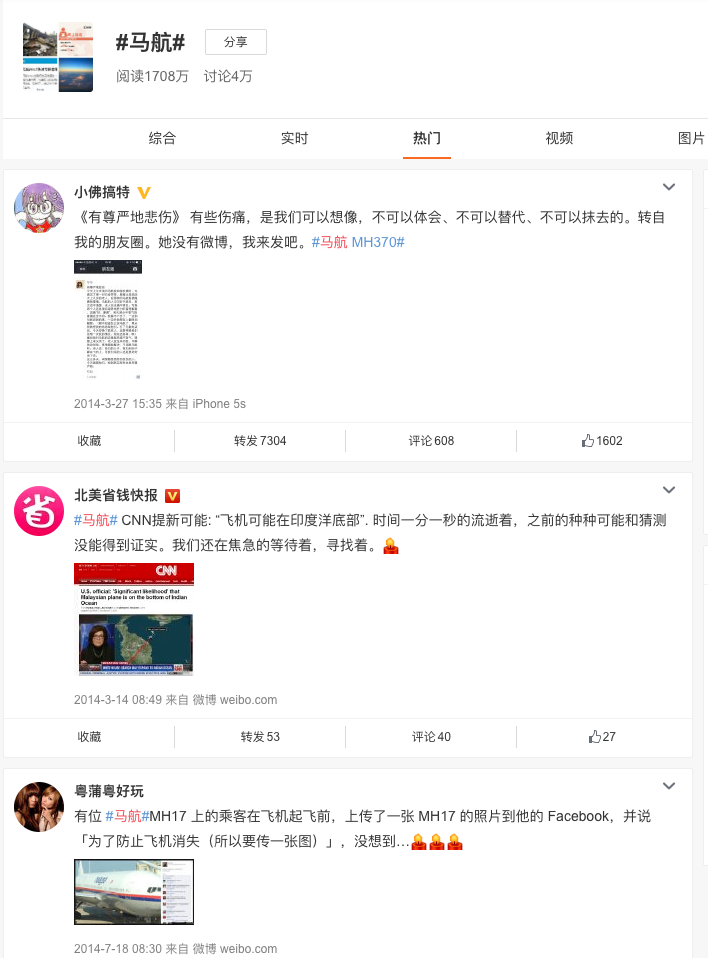
\includegraphics[width=\textwidth]{hashtag_popularity_a}

      \label{fig:hashtag_popularity_a}
    \end{subfigure}%
    ~%add desired spacing
    \begin{subfigure}[b]{0.5\textwidth}
      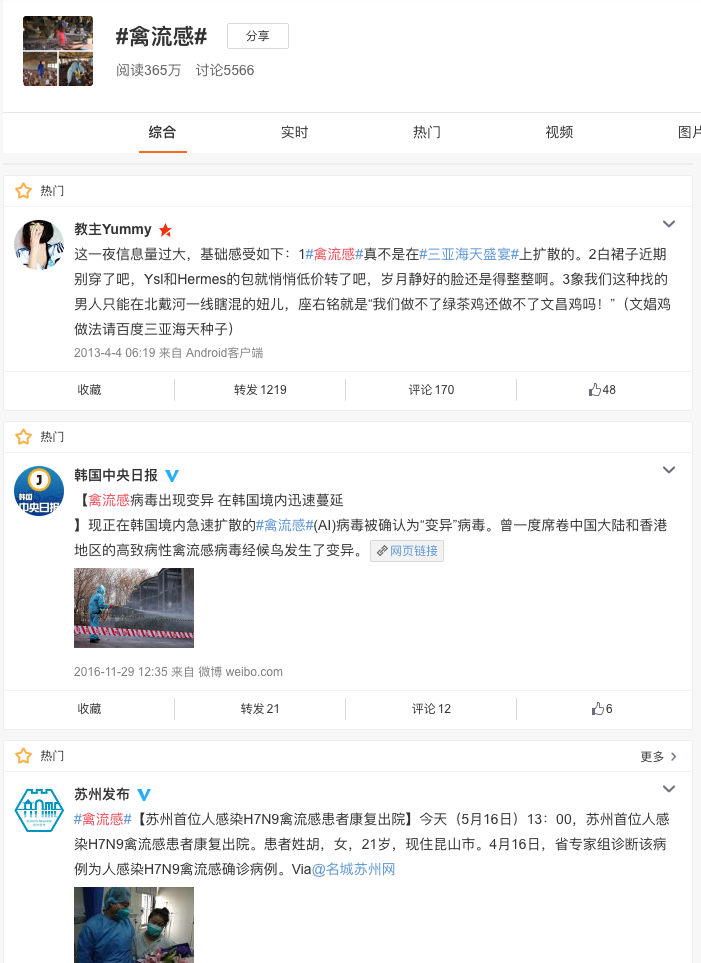
\includegraphics[width=\textwidth]{hashtag_popularity_b}

      \label{fig:hashtag_popularity_b}
    \end{subfigure}
    \bicaption{不同 Hashtag 的阅读数以及出现情况}{Readings And Occurrences Of Different Hashtag}
    \label{fig:hashtag_popularity}
\end{figure}
在本文中,使用 Hashtag 在微博消息中出现的次数来表示该 Hashtag 的流行 度,原因如下:\begin{enumerate}
\item 当用户在一条微博消息中添加 Hashtag 的时候,表示用户对此 Hashtag 的 认可,这个操作真实的表达了用户的主观意见;
\item 是否为热点话题是一个二值化的属性,即“是”与“不是”,可以对应“流行” 与“不流行”,但是不能完整的体现“度”的概念,而出现的次数是一个数值化的属 性,则能更好地表现流行的“程度”;
\end{enumerate}

因此,本文使用 Hashtag 在微博中出现的次数来代表其流行度,进行预测。

\section{问题描述和基本思路}

\subsection{问题描述}

本章所要研究的主要是根据历史上 Hashtag 出现的情况,预测未来某时刻内 Hashtag 出现的频率,具体是根据 Hashtag 过去连续两周的数据预测接下来一天 内 Hashtag 出现的次数,模型预测的结果要尽量和真实数值接近,Hashtag 出现 次数时间分布如图\ref{fig:3_1}所示,由图可知大部分的 Hashtag 的存活时间是超过两周 的,因此该预测问题是有效的。

\begin{figure}[H]
    \centering
    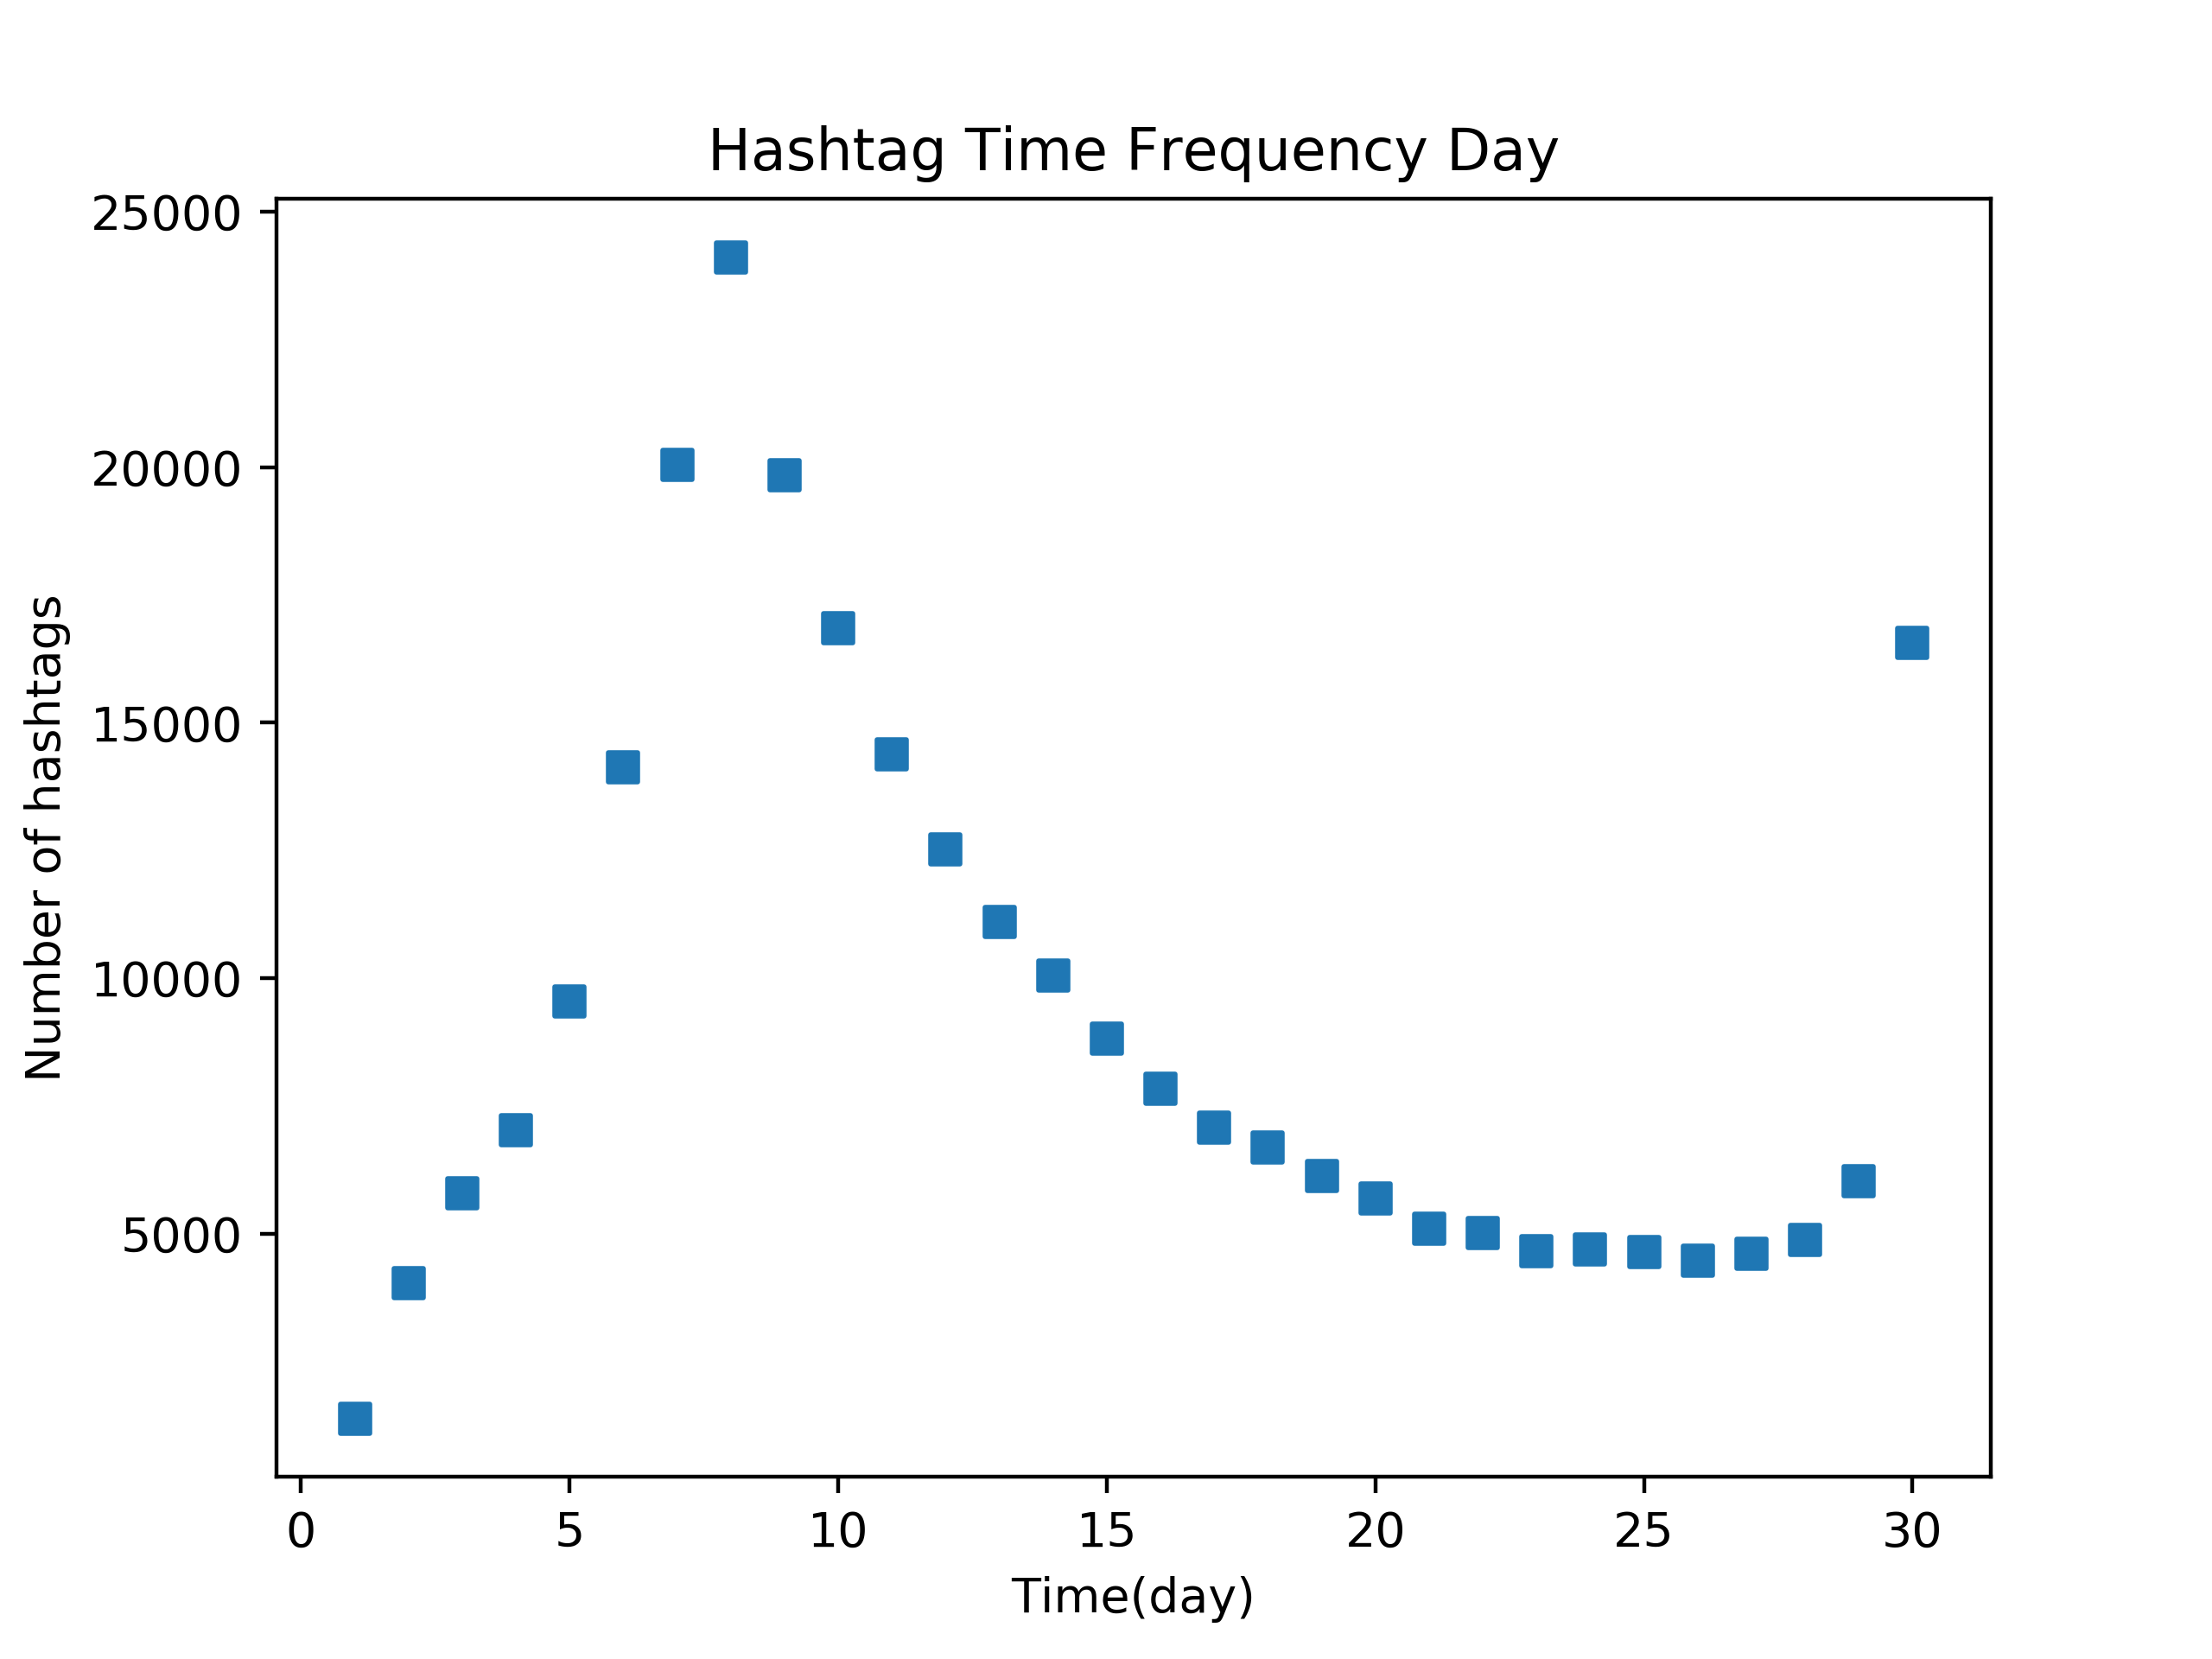
\includegraphics[width=0.5\textwidth]{hashtag_time_new_1}
    \bicaption{Hashtag 时间次数分布图}{Hashtag Time Distribution Chart}
    \label{fig:3_1}
\end{figure}

\subsection{基本思路}
现有的社交网络中的 Hashtag 流行度预测问题没有考虑用户之间的社交网络 结构以及 Hashtag 自身的特性。当前的流行度预测问题,主要考虑的是 Hashtag 的时间序列特征以及 Hashtag 的内容特征,例如考虑时间间隔内 Hashtag 的转发 次数,来预测接下来的转发情况,当然时间序列特征是一个直观并且比较有效的 特征,它很好的反映了消息一个时间段内的热门程度。但是 Hashtag 本身是由用 户产生并且进行转发的,用户之间的关注关系是十分重要。并且 Hashtag 有其自 身特性,比如情感性,地域性以及事件性,这些都是其自身重要的特征,对于预 测 Hashtag 的流行度具有很大作用。因此,本文希望在现有的特征的基础上考虑 用户的粉丝网络结构特征以及 Hashtag 的自身特性,更好的进行 Hashtag 流行度 预测。

因此,本章的基本思路是考虑原有的时间序列等特征,结合用户的粉丝网络 结构特征,学习每个用户的向量表示,刻画用户特征。同时考虑 Hashtag 自身特 性,考虑其情感性以及地域性,构建 Hashtag 不同消息的重要特征。在此特征的 基础上,采用多种机器学习模型,进行 Hashtag 流行度预测的实验。

由于本章所使用的特征涉及用户粉丝网络结构表示以及主题模型,所以首 先对这两部分的内容进行说明,便于后续特征工程的展开。

\section{⺴络表示学习}
网络表示学习(Representation Learning on Network),通常来说就是网络的
向量化技术,简单来说,即将网络中的结构(节点、边或者子图),通过一系列
 过程,变成一个多维向量,通过这样的操作,能够将复杂的网络结构信息变成结 构化的多维特征,实现可计算的向量表示,从而利用机器学习方法实现更方便的 算法应用。

\subsection{基于 DeepWalk 的用户粉丝网络表示}

Deepwalk 是 2014 年发表在 KDD 上的一篇论文 \citep{Perozzi2014DeepWalk},这篇文章受到了词向量 学习模型 word2vec 的启发,文章的思路就是对网络应用了 word2vec 的 SkipGram 模型。SkipGram 模型原本是针对文本数据进行学习的,或者说是针对有序序列 的,因此 Deepwalk 先应用随机游走得到网络中的一些列有序的节点序列,这些 节点序列类似于文本中的句子,通过这样的数据处理方式,将这些“句子”使用 SkipGram 模型进行训练,从而得到“句子”中每个“单词”的向量表示,结果数据展 示如图\ref{fig:piu_0}所示。
\begin{figure}[!htbp]
    \centering
    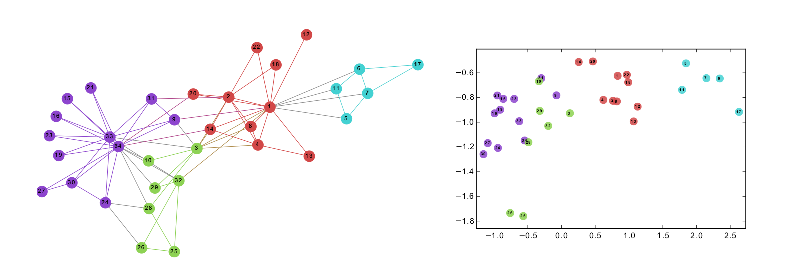
\includegraphics[width=0.7\textwidth]{dw}
    \bicaption{DeepWalk 数据展示 \citep{Perozzi2014DeepWalk}}{DeepWalk Show\citep{Perozzi2014DeepWalk}}
    \label{fig:piu_0}
\end{figure}


Deepwalk 的随机游走过程事实上是对网络结构进行随机采样的过程,将网 络中的节点通过随机游走的方式表示出来,两个节点联系越紧密,在一个随机游 走过程中共同出现的可能性越大,反之若两个节点根本不连通,则随机游走的方 式是不可能将两个节点共同出现的。因此 Deepwalk 能很好的将网络的连接情况 进行表示,且实验证明在网络规模较大时具有很高的效率,其算法流程如\ref{alg:DeepWalk_1}和\ref{alg:SkipGram_1}。

\begin{algorithm}[H]
\renewcommand{\algorithmicrequire}{\textbf{Input:}} 
\renewcommand{\algorithmicensure}{\textbf{Output:}}
    \small
    \caption{DeepWalk(G,$\omega$,d,$\gamma$,t)}
    \label{alg:DeepWalk_1}
    \begin{algorithmic}
    \Require graph G(V,E) \\
    window size $\omega$ \\ 
    embedding size d \\
     walks per vertex $\gamma$ \\ 
     walk length t 
     \Ensure{matrix of vertex representations $\Phi$ $\in$  $R^{|V|{\times}d}$}
     
      \State $ Initialization: Sample ~\Phi from U^{|V |d}$
      \State $Build~ a~ binary ~Tree~ T ~from~ V $
       \For {i~=~0 to $\gamma$} 
			\State $O = Shuffle(V ) $
			\For  {${v_i}$~ $\in$~O}
				\State $W_{v_i} = RandomWalk(G,v_i,t)$
				\State $SkipGram(\Phi, W_{v_i} , w)$
			\EndFor
		\EndFor
    \end{algorithmic}
\end{algorithm}

\begin{algorithm}[H]
    \small
    \caption{SkipGram($\Phi$,$\Omega_{v_i}$,$\omega$)}\label{alg:SkipGram_1}
    \begin{algorithmic}[1]
       \For {${v_j}$ $\in$ $\Omega$} 
			\For  {${u_k}$~ $\in$~$\Omega_{v_i}[j - w : j + w]$}
				\State $J(\Phi) = -\log Pr(u_k|\Phi(v_j))$
				\State $\Phi = \Phi - \alpha * \frac{\partial J}{\partial \Phi}$
			\EndFor
		\EndFor
    \end{algorithmic}
\end{algorithm}

其大致思想就是用随机游走蒙特卡罗采样,然后送到 word2vec 去训练,最 终得到每个节点的向量表示,训练方式如图\ref{fig:piu_1}所示。


\begin{figure}[H]
    \centering
    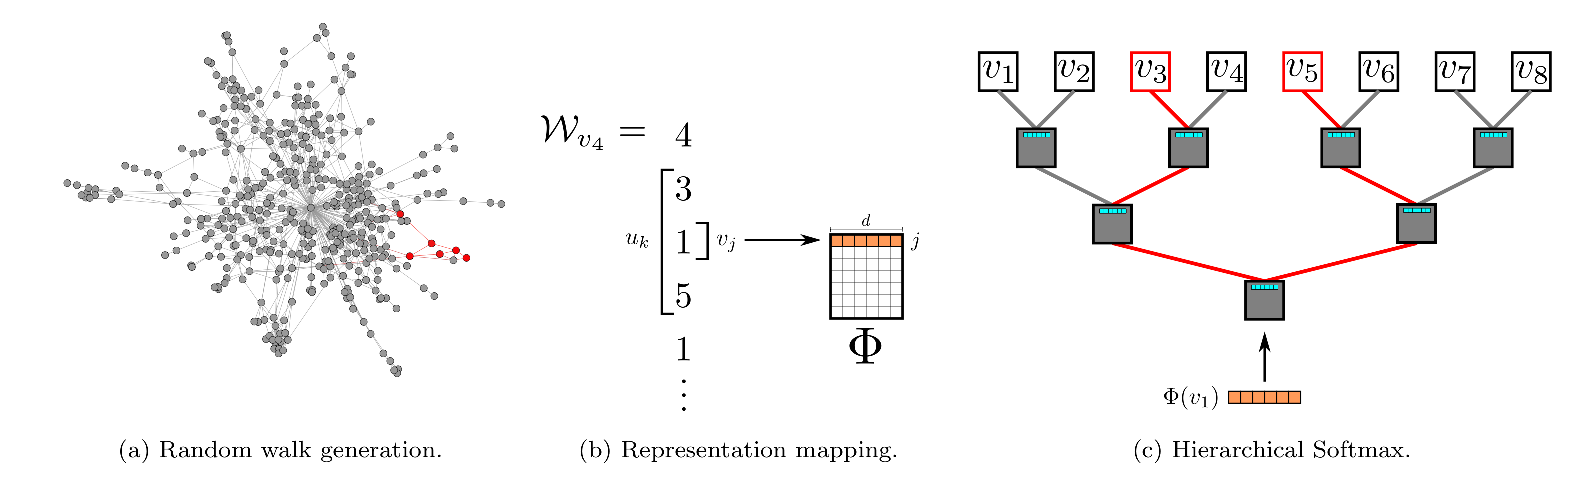
\includegraphics[width=0.7\textwidth]{hashtag_1}
    \bicaption{DeepWalk训练过程\citep{Perozzi2014DeepWalk}}{DeepWalk Training Process\citep{Perozzi2014DeepWalk}}
    \label{fig:piu_1}
\end{figure}

\subsection{基于 LINE 的用户粉丝网络表示}
LINE 是 2015 年提出的一种网络结构表示学习方法,该方法提出了一阶邻 近度与二阶邻近度的概念,基于这两个邻近度,提出了优化函数,得到的最优化 结果即为每个节点的向量表示\citep{Tang2015LINE}。

该方法的优化过程可以理解为基于两个假设:
\begin{enumerate}


\item 直接相连的节点表示尽可能相近(一阶邻近度),它们的距离尽可能的 小,如图\ref{fig:piu_2}中的节点 6 和节点 7。文中两个节点的联合概率表示其一阶邻近度, v 代表节点,u 代表节点的 embedding。公式\ref{eq:line_1}的意思是两节点越相似,内积越 大,sigmoid 映射后的值越大,也就是这两节点相连的权重越大,也就是这两个 节点间出现的概率越大。

\begin{equation}\label{eq:line_1}
	p_1(v_i,v_j) = \frac{1}{1 + \exp(-\overrightarrow{u_i}^{T} ~\cdot~ \overrightarrow{u_j})}
\end{equation}

\item 两个节点公共的邻居节点越多,两个节点的表示越相近(二阶邻近度),
如图\ref{fig:piu_2}中的节点 5 和节点 6。公式\ref{eq:line_2}用两个节点的条件概率表示其二阶邻近度。

\begin{equation}\label{eq:line_2}
	p_2(v_i|v_j) = \frac{\exp(\overrightarrow{u_j}^{\prime T}~\cdot~\overrightarrow{u_i})}{\begin{matrix}
	\sum_{k=1}^V ~\exp(-\overrightarrow{u_k}^{\prime T} ~\cdot~ \overrightarrow{u_j})
\end{matrix}	 }
\end{equation}


\end{enumerate}

\begin{figure}[H]
    \centering
    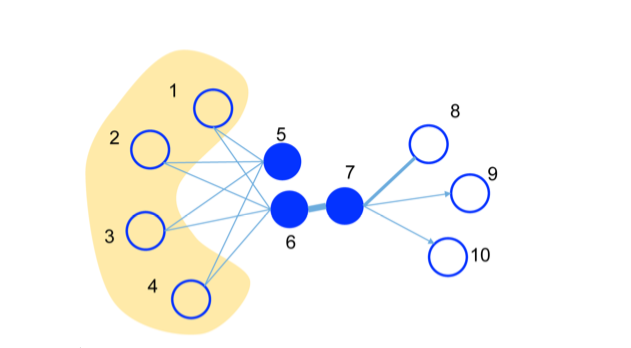
\includegraphics[width=0.7\textwidth]{hashtag_}
    \bicaption{用户网络结构图\citep{Tang2015LINE}}{User Network Structure\citep{Tang2015LINE}}
    \label{fig:piu_2}
\end{figure}

\subsection{小结}
对比网络表示学习中的 DeepWalk 和 LINE 等算法的原理,考虑到 LINE 算
法提出了一个明确的目标函数,问题可以进行直接优化,对于网络表示学习有更
 好的结果,因此本文的用户粉丝网络结构表达采用 LINE 的方式进行学习,通过 明确的优化方式,用户的向量表达更加准确。

\section{主题模型}
在人们日常获取信息的方式上,文本占有很大分量,为了更快更精确地从大 量的文本数据中取得所需要的信息,针对文本信息处理的研究一直在进行。文本 数据不光信息量大,而且一般是无结构的。另外,通常的文本数据以矩阵的形式 被计算机处理,此时的数据矩阵具有高维稀疏的特征,空间占用较大,因此,对 大规模文本信息进行处理分析的另一个障碍便是如何削减原始数据的维度。


\subsection{NMF 非负矩阵分解}
通常的矩阵分解会把一个大的矩阵分解为多个小的矩阵,但是这些矩阵的 元素有正有负。而在现实世界中,文本数据等形成的矩阵中负数的存在是没有 意义的,因此如果能把一个矩阵分解成全是非负元素的矩阵是很有价值的。在 NMF 中要求原始矩阵中的所有元素均是非负的,那么矩阵可以分解为两个更小 的非负矩阵的乘积,这个矩阵有且仅有一个这样的分解,即满足存在性和唯一性\citep{Du2010Nonnegative}。

NMF 的思想:V=WH(W 权重矩阵、H 特征矩阵、V 原矩阵),通过计算从 原矩阵提取权重和特征两个不同的矩阵出来,NMF 属于一个无监督学习的算法, 其中限制条件就是 W 和 H 中的所有元素都要大于等于 0。

\begin{figure}[H]
    \centering
    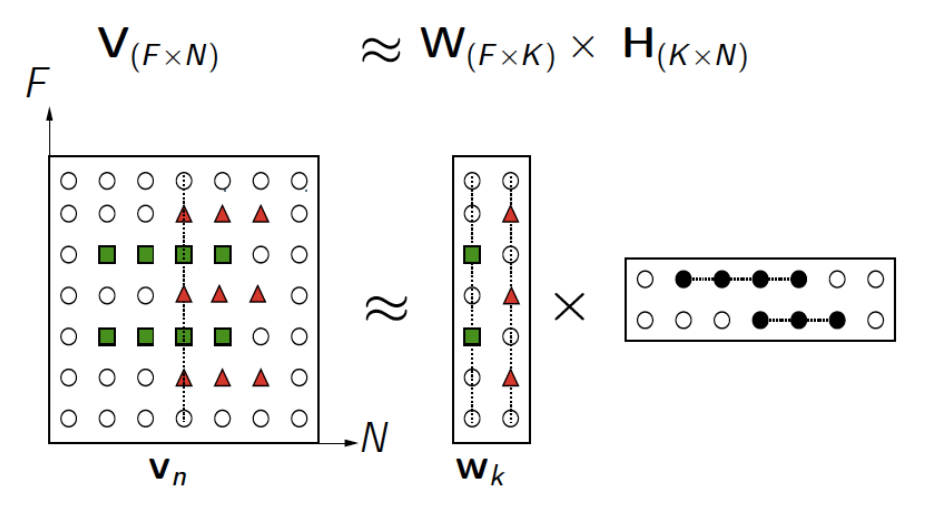
\includegraphics[width=0.5\textwidth]{hashtag_2}
    \bicaption{NMF矩阵分解示意图}{NMF Matrix Decomposition Diagram}
    \label{fig:piu_5}
\end{figure}

\subsection{LDA 主题模型}

LDA(Latent Dirichlet Allocation)是一种文档主题生成模型,也称为一个三层贝叶斯概率模型,包含词、主题和文档三层结构 \citep{Blei2003Latent}。所谓文档主题生成模型,
 就是认为一篇文章中的每个词都是通过“以一定概率选择了某个主题,并从这个 主题中以一定概率选择某个词语”这样一个过程得到的。文档到主题服从多项式 分布,主题到词服从多项式分布。
 
LDA 是一种非监督机器学习技术,可以用来识别大规模文档集(document collection)或语料库(corpus)中潜藏的主题信息。它采用了词袋模型(bag of words)的方法,这种方法将每一篇文档视为一个词频向量,从而将文本信息转 化为了易于建模的数字信息。词袋方法没有考虑词与词之间的顺序,这简化了问 题的复杂性,同时也为模型的改进提供了方向。每一篇文档代表了一些主题所构 成的一个概率分布,而每一个主题又代表了很多单词所构成的一个概率分布。

LDA 主题模型主要是对文档词矩阵进行降维,数据输入如图\ref{fig:piu_6}所示。

\begin{figure}[H]
    \centering
    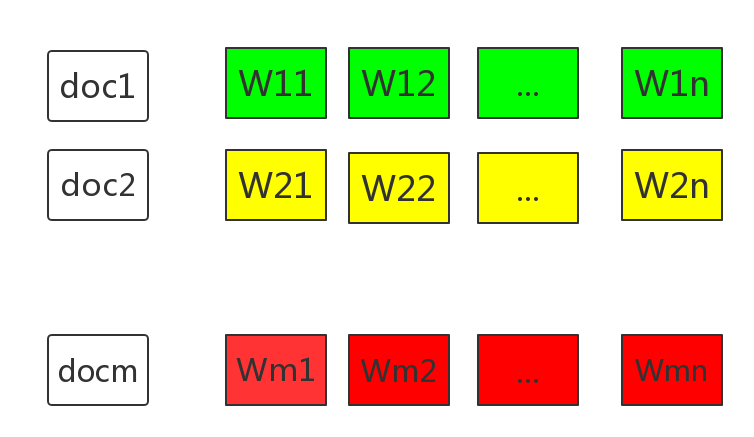
\includegraphics[width=0.5\textwidth]{lda}
    \bicaption{LDA文档词矩阵}{LDA Document Word Matrix}
    \label{fig:piu_6}
\end{figure}


LDA 模型的目标是找到每一篇文档的主题分布和每一个主题中词的分布。 在 LDA 模型中,我们需要先假定一个主题数目 K,这样所有的分布就都基于 K 个主题展开, 具体过程如图\ref{fig:piu_7}所示。
\begin{figure}[H]
    \centering
    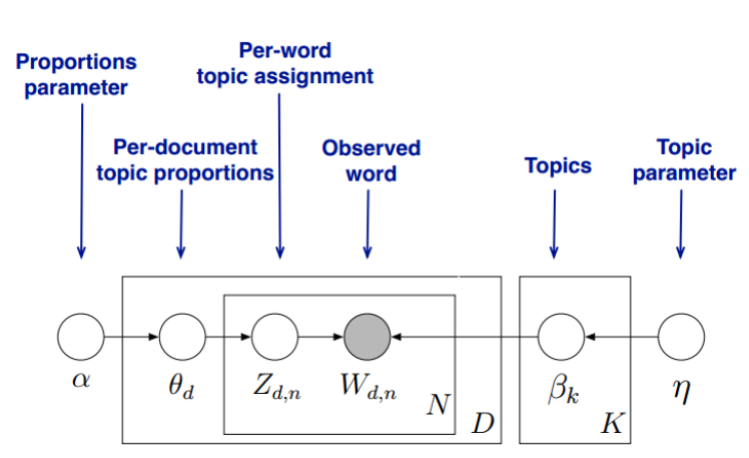
\includegraphics[width=0.5\textwidth]{hashtag_4}
    \bicaption{LDA主题模型流程图}{LDA Flow Chart}
    \label{fig:piu_7}
\end{figure}

\section{Hashtag数据特点}

如在相关研究中所述,在消息流行度预测领域有很多已有的研究成果,比 如对微博中热门话题的发现和预测等,其中的一些方法可以直接应用在本文所 要研究的问题上,但这些研究成果因为没有考虑到 Hashtag 流行度预测的场景特 点,都有提高的空间。

在进行 Hashtag 流行度预测之前,本文首先分析其出现频次的特征,从宏观 角度考察数据分布情况,对于后期特征的提取以及模型的优化有较大的指导意 义。

相比于微博消息的流行度预测,Hashtag 流行度预测与其存在一些共性,比 如它们的分布都是呈现幂律分布的,如图\ref{fig:piu_8}所示,因此消息预测中的一些特性, 比如时间序列特征很显然可以适用到 Hashtag 的流行度预测中。


\begin{figure}[H]
    \centering
    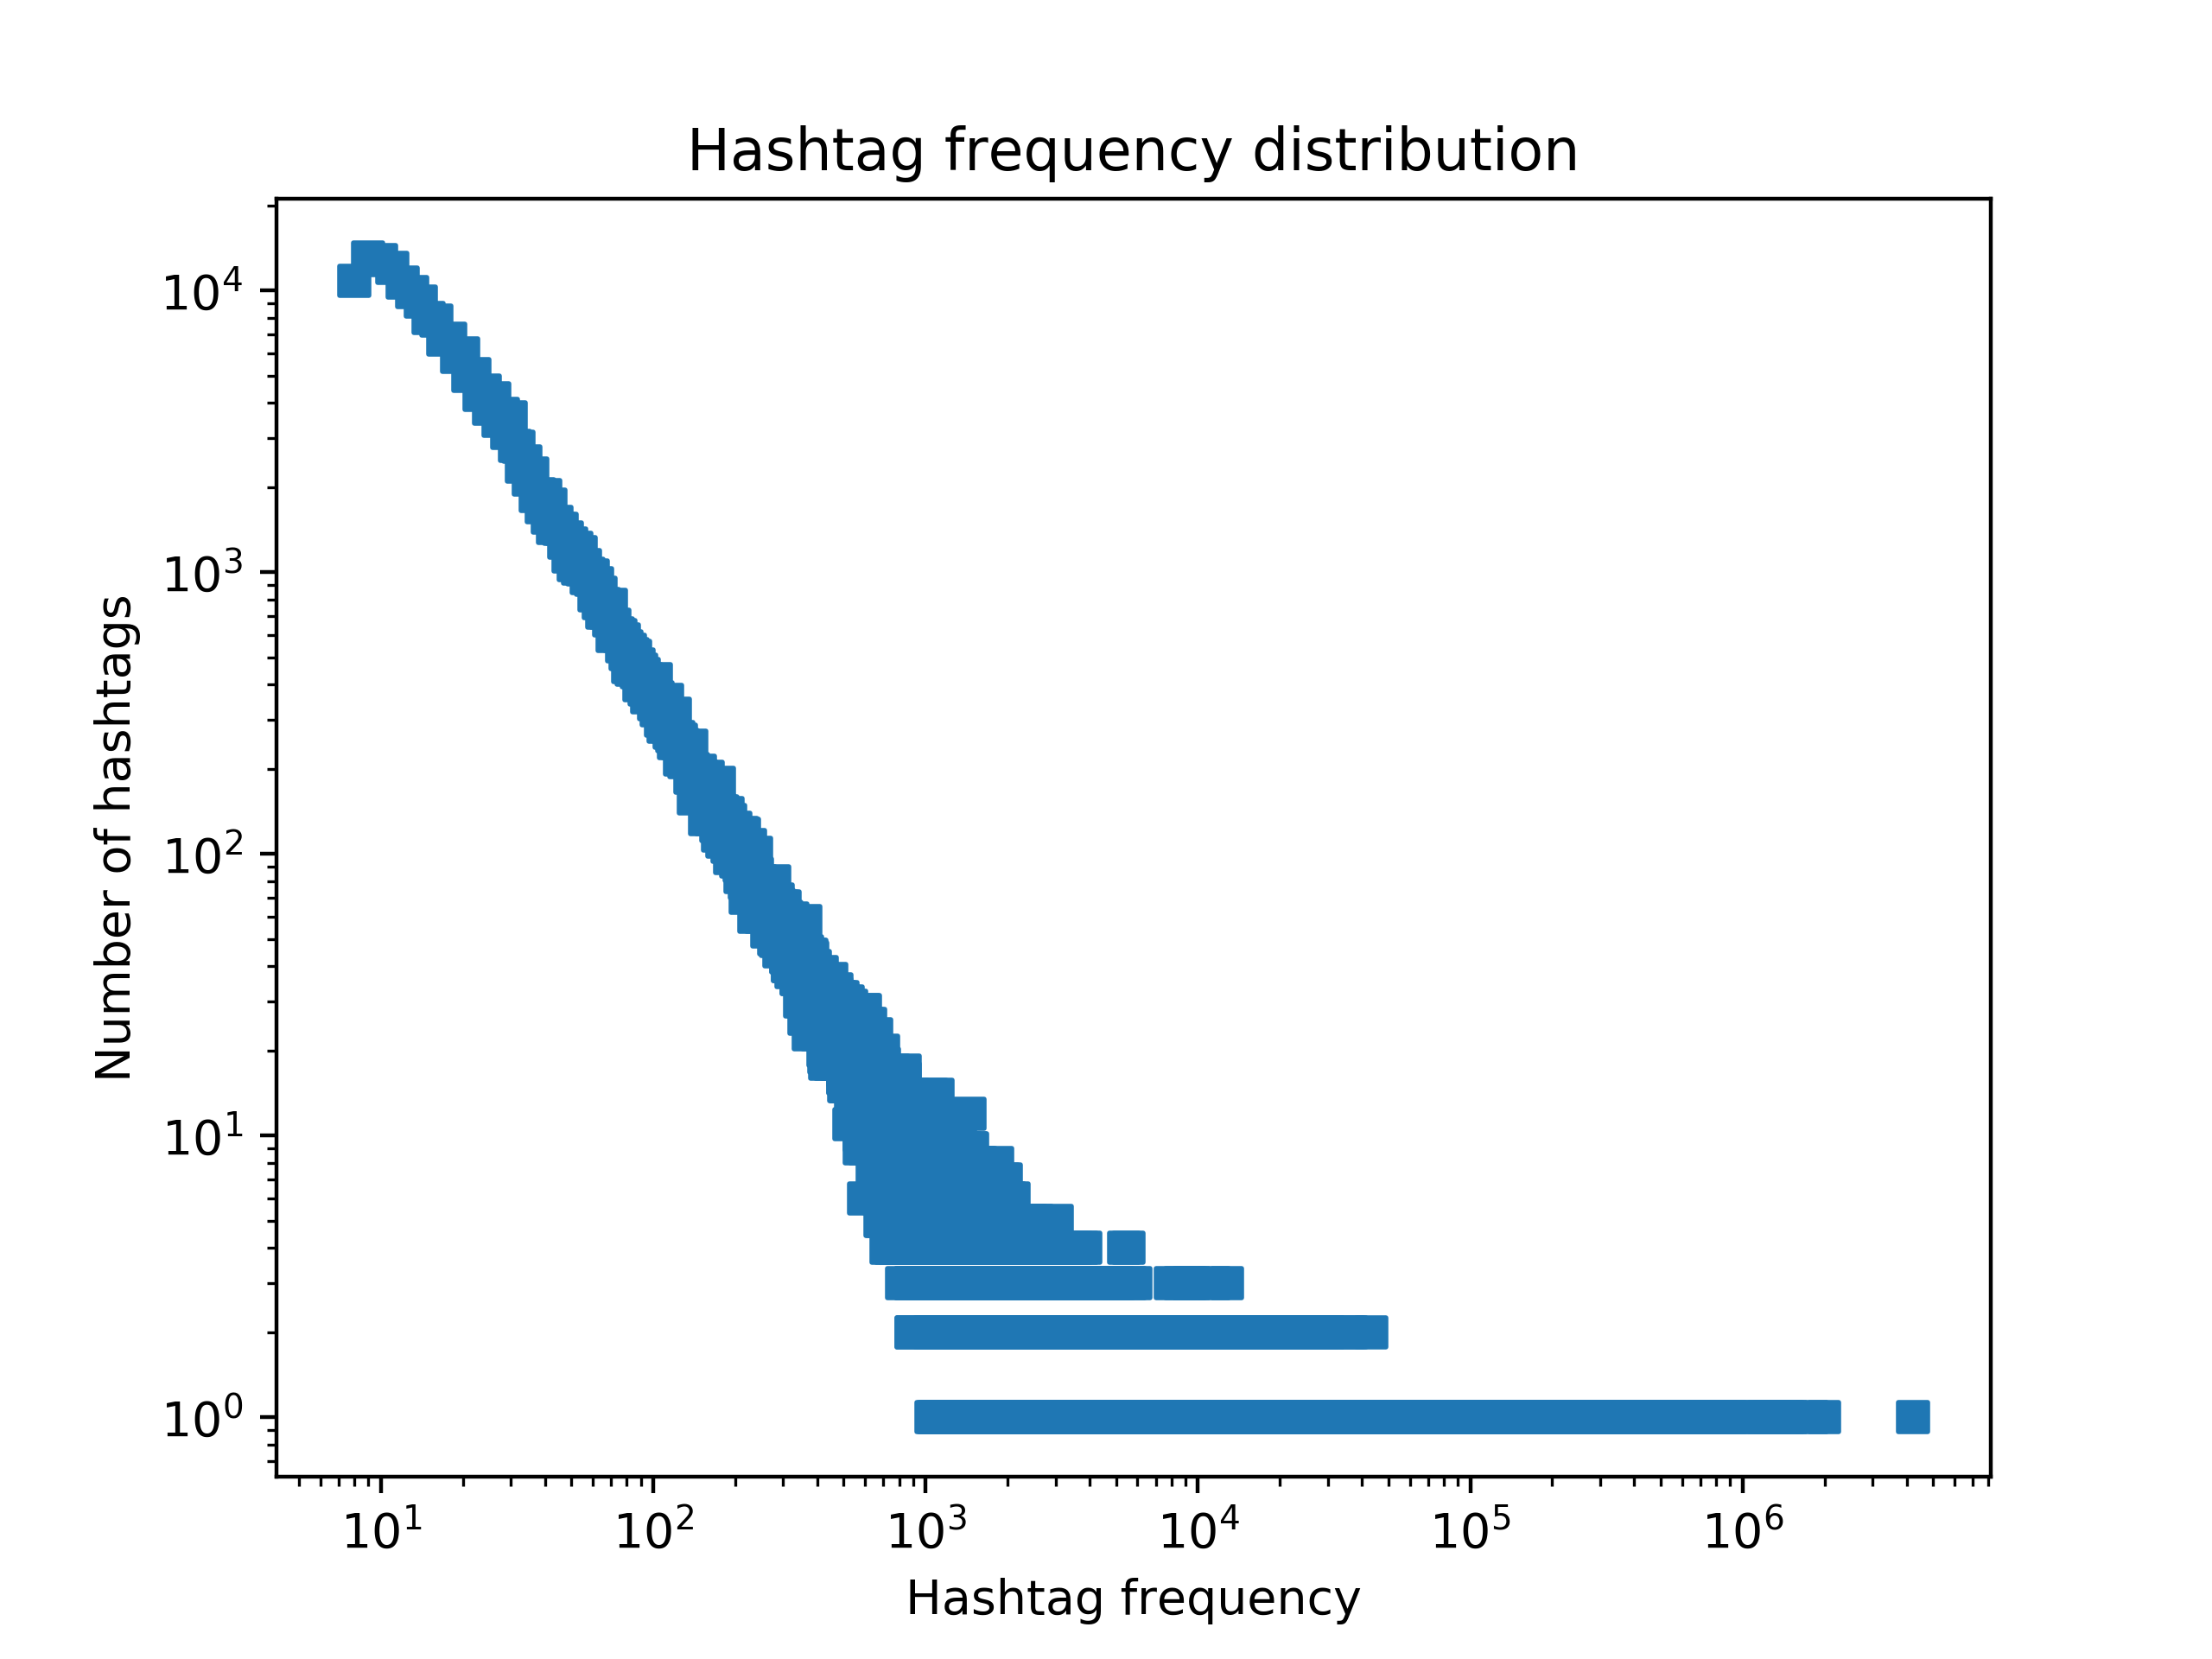
\includegraphics[width=0.5\textwidth]{hashtag_5}
    \bicaption{Hashtag分布情况}{Hashtag Distribution}
    \label{fig:piu_8}
\end{figure}


但是 Hashtag 自身存在许多消息不存在的特性,Hashtag 本身可以作为一个 事件或者一个话题,其带有鲜明的主观意愿,而微博消息本身对于事件的表述 不是很准确,无法从单一的微博消息获得深入的认识,而 Hashtag 短短几个字就 抓住了用户的想法,所以它们之间存在很大区别。比如对于 \# 李小璐出轨 \# 这个 Hashtag,如图\ref{fig:lixiaolu}所示,它的流行度预测受标签本身的特性影响很大,比如里面 出现的公众人物,情感色彩,地域信息等等,而这些在微博消息中都是很难捕捉 到的。


\begin{figure}[!htbp]
    \centering
    \begin{subfigure}[b]{0.5\textwidth}
      
\includegraphics[width=\textwidth]{l_1}
      \caption{}
      \label{fig:oaspl_a}
    \end{subfigure}%
    ~%add desired spacing
    \begin{subfigure}[b]{0.5\textwidth}
      
\includegraphics[width=\textwidth]{l_2}
      \caption{}
      \label{fig:oaspl_b}
    \end{subfigure}
    \begin{subfigure}[b]{1\textwidth}
      
\includegraphics[width=\textwidth]{l_3}
      \caption{}
      \label{fig:oaspl_c}
    \end{subfigure}%
    ~%add desired spacing
    \bicaption{\# 李小璐出轨 \#Hashtag 传播示意图}{Hashtag communication diagram}
    \label{fig:lixiaolu}
\end{figure}

\section{特征空间}
本文对于 Hashtag 流行度预测所提的特征主要包括内容特征,时间序列特 征,用户粉丝网络结构特征,Hashtag 自身特性以及微博用户特性等,下面对于 每种特征进行详细说明。

\subsection{内容特征}

\subsubsection{微博消息的统计特征}
Hashtag 本身是存在于微博消息中的,所以这部分特征主要是微博消息的统 计特征。
\begin{enumerate}
\item 微博消息分词后的单词数量,以及 hashtag 在这些单词中出现的比例,来 表明它们之间的相关性;
\item 微博消息中是否包含 URL 链接,URL 链接的数量,占消息的比例,因为 带有链接的消息内容更加丰富,更容易转发;
\item 微博消息中表情符号出现的次数,这些特征容易引起用户的关注;
\end{enumerate}

\subsubsection{微博消息的特征}
\begin{enumerate}
\item 微博消息的主题特征,本文对微博消息抽取 TF-IDF 关键词,然后采用 NMF 非负矩阵分解以及 LDA 进行训练学习,分别选取三十维向量来获取微博 消息的主题表达;
\item 微博消息的情感性,以及正负中性出现的比例;
\item 微博消息的类型数量以及比例;
\end{enumerate}


\subsection{时间序列特征}

这部分主要是统计每一时间段内的 Hashtag 出现的次数,作为一个连续的时 间序列特征,以及这段序列特征的平均数,中位数和方差,时间序列特征是对流 行度的最直观的表述,这部分的影响一般是很重要的。

\subsection{Hashtag 自身特征}

\begin{enumerate}
\item Hashtag 分词后的单词数量以及其所有字符的长度;
\item Hashtag是否包含数字,因为数字很可能是某个特殊标识,比如节日等等; 
\item Hashtag 是否包含人名,带有人名的 Hashtag 很可能是某些公众人物,这
样的标签更容易引起人们关注;
\item Hashtag 标签的情感性,来反映用户的直观感受;
\end{enumerate}


\subsection{微博的地域特征}
由于网民关注的事件带有很强的地域性信息,不同地域的人关注的主题不 同,比如在民间文化上,北京地区的可能关注的是京剧,而东北可能关注的是带 有地域特色的东北二人转,因此综合考虑地域信息,将微博消息按照地域划分, 可以进行简单的群体聚类,将相似的事物进行共同处理,具体特征划分如下:
\begin{enumerate}
\item 微博消息的地域信息,统计全国每个省以及海外地区出现的次数,将微 博消息按照省级进行划分,考虑省级的地域聚类。
\item 微博消息的地域信息,进行全国地区的划分,将全国分为九个大的地区, 来获取地域整体的信息,比如东三省的消息之间的相似度可能比较高,进行多省 间的地域聚类。
\end{enumerate}


\subsection{微博用户自身特征}
\begin{enumerate}
\item 原发消息的微博用户的粉丝数以及朋友数,来反映初始消息可能转发的 可能性;
\item 转发消息的微博用户的粉丝数以及朋友数,来反映此时消息的关注程度;
\end{enumerate}



\subsection{用户粉丝网络结构特征}
本文考虑 Hashtag 的产生和转发都是用户主导的,因此微博用户粉丝之间的 网络结构信息是十分重要的,本文采用网络结构表示方法对于用户粉丝网络结 构进行 Embedding 学习,来表示用户向量,既可以对用户粉丝网络进行直观表 示,便于计算,同时又降低了向量维度。本文采用 LINE 对于用户粉丝网络结构 进行学习,每个用户表示成一个 100 维的向量,然后进行模型训练。

\section{特征抽取与模型实现}

\subsection{sklearn 介绍}

本文的特征抽取以及机器学习模型都是使用 sklearn 实现的 \citep{Komer2014Hyperopt}。sklearn 是 机器学习中一个常用的 python 第三方模块,里面对一些常用的机器学习方法进 行了封装,在进行机器学习任务时,并不需要每个人都实现所有的算法,只需要 简单的调用 sklearn 里的模块就可以实现大多数机器学习任务。

机器学习任务通常包括分类(Classification)和回归(Regression),常用的 分类器包括 SVM、KNN、贝叶斯、线性回归、逻辑回归、决策树、随机森林、 xgboost、GBDT、boosting、神经网络 NN。常见的降维方法包括 TF-IDF、主题
 模型 LDA、主成分分析 PCA 等等,sklearn 均有实现, 方便用户快速实现其想法。 并且里面包含一些常见的特征提取方法,对于提取文本,图像特征都可以,为 用户高效提取数据特征提供了便利。sklearn 里面自带了很多算法包的评价指标, 对于模型的有效性以及特征的重要性都可以方便评估。
 
综上所述,sklearn 的出现大大方便了机器学习者们快速的部署自己的模型, 用于机器学习和深度学习方面的研究。本文的模型部署在 sklearn-0.19.0 上,特 征提取基本也是使用其实现,整个特征提取以及模型训练过程只需要大约 4 个 小时就可以完成。


\subsection{模型训练}

本文进行的 Hashtag 流行度预测是一个回归任务,因此本文选用了回归任务 效果比较好的 SVM, 随机森林以及 xgboost 模型来完成该任务。对于 SVM 模型 参数,本文采用了线性核来进行训练,而对于随机森林和 xgboost 这种都是树模 型,因此它们之间存在许多共同参数,参数如表\ref{tab:3_1}所示。

\begin{table}[H]
    \centering
    \footnotesize% fontsize
     \bicaption{树模型主要参数}{Tree model main parameters}
      \label{tab:3_1}
    \setlength{\tabcolsep}{30pt}% column separation
    \renewcommand{\arraystretch}{1.2}%row space 
    \begin{tabular}{ccc}
        \hline
        \textbf{编号} & \textbf{模型参数} & \textbf{含义} \\
        %\cline{2-9}% partial hline from column i to column j
        \hline
         1 & $n\_estimators$ & 树的个数 \\
         2 & $max\_depth$ &  树的深度\\
         3 & $eta$ & 学习率\\
         4 & $subsample$ & 采样\\ 
        	\hline
    \end{tabular}
    
\end{table}


\section{实验结果与分析}

本文使用 3.6 节提出的 Hashtag 特征进训练,模型采用 SVM、随机森林和 xgboost, 将不包括 Hashtag 自身特性以及用户粉丝网络结构特征作为 baseline,然 后进行全部特征的模型训练,并对实验结果进行分析。

\subsection{实验数据}
\subsubsection{微博消息数据}
在机器学习中,为了让模型学习到更多有用的特征,保持数据的多样性和差 别性,往往需要大量的训练样本,这样可以提高模型的鲁棒性以及实验效果。本 文采集了一个月的微博数据,数据量大概两亿条,从这些数据中构建了 Hashtag的训练和测试样本。

\begin{table}[H]
    \centering
    \footnotesize% fontsize
     \bicaption{微博数据}{Weibo data}
      \label{tab:3_2}
    \setlength{\tabcolsep}{30pt}% column separation
    \renewcommand{\arraystretch}{1.2}%row space 
    \begin{tabular}{ccc}
        \hline
        \textbf{编号} & \textbf{属性} & \textbf{属性值} \\
        %\cline{2-9}% partial hline from column i to column j
        \hline
         1 & 文件大小& $130G$ \\
         2 & 微博消息数量& $200000000$\\
         3 & Hashtag 数量& $5923117$ \\
        	\hline
    \end{tabular}
    
\end{table}

\subsubsection{Hashtag 数据}
通过对微博数据进行解析分析,剔除掉出现频率过低的 Hashtag 样本(连续 15 天出现次数小于 15 次),根据前面的特征空间,抽取相应的特征数据,生成 训练样本进行模型训练。
\begin{table}[H]
    \centering
    \footnotesize% fontsize
         \bicaption{Hashtag训练数据}{Hashtag training data}
      \label{tab:3_3}
    \setlength{\tabcolsep}{30pt}% column separation
    \renewcommand{\arraystretch}{1.2}%row space 
    \begin{tabular}{ccc}
        \hline
        \textbf{编号} & \textbf{属性} & \textbf{属性值} \\
        %\cline{2-9}% partial hline from column i to column j
        \hline
         1 & 文件大小 & $1.1G$ \\
         2 &训练样本数据& $370633$\\
         3 & 特征类型数量 & $7$ \\
         4 &微博特征维度& $7$\\
       	5 &Hashtag 特征维度& $4$\\
       	6 &时间序列特征维度& $30$ \\
       	7 & 区地域特征维度& $8$\\
       	8 &省地域特征维度& $35$\\
       	9 &主题特征维度& $60$\\
       	10 & 用户向量表示维度 & $100$\\
       	11&用户自身特征维度& $2$\\

        	\hline
    \end{tabular}

\end{table}

\subsubsection{用户粉丝网络数据}
另外对于用户粉丝网络结构,本文社交关系网络包含一个约 256.7w 微博用 户的社交网络,里面存在 5.5 亿条关注关系,对于充分学习用户粉丝网络结构表 达是足够的。

\begin{table}[H]
    \centering
    \footnotesize% fontsize
        \bicaption{用户粉丝网络结构数据}{User fan network structure data}
      \label{tab:3_4}
    \setlength{\tabcolsep}{30pt}% column separation
    \renewcommand{\arraystretch}{1.2}%row space 
    \begin{tabular}{ccc}
        \hline
        \textbf{编号} & \textbf{属性} & \textbf{属性值}\\
        %\cline{2-9}% partial hline from column i to column j
        \hline
         1 &文件大小 & $5.6$ \\
         2 & 具有粉丝的用户数量 & $1671145$\\
         3 & 用户总量 & $2529073$ \\
         4 &用户粉丝连接边的数量& $550000000$ \\ 
        	\hline
    \end{tabular}
 
\end{table}



\subsection{评价指标}

模型在训练数据上进行训练,然后在测试数据上进行验证。针对测试数据中
的每一个 Hashtag,本文预测其未来的流行度,采用如下评价指标进行评估:

MSE(Mean Squared Error) 均方误差是回归问题的常用指标, 公式如\ref{eq:mse}所示, 它是指参数估计值与参数真值之差平方的期望值; MSE 可以评价数据的变化程 度,MSE 的值越小,说明预测模型描述实验数据具有更好的精确度。

 
\begin{equation}\label{eq:mse}
	MSE = \frac{1}{N} ~\sum_{t=1}^N~(observed_t - predicted_t)^2
\end{equation}

 
MAE(median absolute error)公式如\ref{eq:mae}所示,该函数尤其有趣,因为它的离群值很强. 通过取目标和预测之间的所有绝对差值的中值来计算损失。
  
  \begin{equation}\label{eq:mae}
  MAE = median(|observed_1 - predicted_1|,...,|observed_N - predicted_N|)
  \end{equation}
  
MSLE(mean squared log error) 公式如\ref{eq:msle_3}所示, 函数计算了一个对应平方对数 (二次)误差或损失的预估值风险度量, 由于 Hashtag 的分布呈现幂率分布,因此
通过 log 运算,该指标更加适合具有指数增长趋势的数据。
 
 \begin{equation}\label{eq:msle_3}
 	MSLE = \frac{1}{N}~\sum_{t=1}^N~(\log{(observed_t + 1)} - \log{(predicted_t + 1)})^2
 \end{equation}
 
\subsection{实验结果}
首先,我们将所有特征在模型之间进行测试,衡量一下不同模型之间的差 异,然后选取结果最好的模型在不同特征集合上的表现,来说明各个特征的重要 性。
\subsubsection{模型间对比}
SVM, 随机森林 (Random Forests) 和 xgboost 的模型预测结果如表\ref{tab:3_5}所示。
\begin{table}[H]
    \centering
    \footnotesize% fontsize
    \bicaption{SVM, 随机森林和 xgboost 结果对比}{Comparison of SVM,RF and xgboost }
      \label{tab:3_5}
    \setlength{\tabcolsep}{15pt}% column separation
    \renewcommand{\arraystretch}{1.2}%row space 
    \begin{tabular}{ccccc}
        \hline
        \textbf{Model} &\textbf{ MSE} & \textbf{MAE} & \textbf{MSLE }& \textbf{Time }\\
        %\cline{2-9}% partial hline from column i to column j
        \hline
         \textbf{SVM} & $4740092.8$ & $6.09$ & $1.6$ & $55800s$ \\
        \textbf{ Random ~Forests } & $1492180.4$ & $5.25$ & $1.09$  & $12647s$ \\
        \textbf{ xgboost }& $1228629.5$ & $4.86$ & $0.97$  & $10237s$ \\
        	\hline
    \end{tabular}
     
\end{table}
 
根据实验结果,本文得到如下结论:
 \begin{enumerate}
\item 从MSE,MAE,MSLE三个指标的整体效果上来看,SVM的结果表现最差, 由于构造的特征数据包含多种类型,而 SVM 对于非线性问题没有通用解决方案, 并且该模型对于缺失数据很敏感,并且该算法的空间消耗和时间消耗都是巨大 的,在大数据量,多维特征上效果不好。
\item 随机森林表现的稍微差点,由于它是一个树模型,能够处理高纬度的特 征数据;在创建随机森林的时候,对 generlization error 使用的是无偏估计,模型 泛化能力强;对于数据的缺失仍有一定的效果,训练速度快,容易做成并行化方 法,因此速度不错。
\item xgboost 模型的效果最好,并且训练用时最少。原因如下:xgboost 在代价 函数里加入了正则项,用于控制模型的复杂度。正则项里包含了树的叶子节点个 数、每个叶子节点上输出的 score 的 L2 模的平方和。从 Bias-variance trade-off 角 度来讲,正则项降低了模型的 variance,使学习出来的模型更加简单,防止过拟 合,这也是 xgboost 优于随机森林的一个特性。并且随机森林在优化时只用到一 阶导数信息,xgboost 则对代价函数进行了二阶泰勒展开,同时用到了一阶和二 阶导数,因此效果在三个模型中最好。 \end{enumerate}
 
\subsubsection{特征重要性之间的对比}
根据特征在各个模型上的整体表现,以及模型之间的优缺点,本文着重分析 不同特征在 xgboost 上的表现,来衡量各个类型特征的重要性,每次去掉其中一 种特征,然后对比其与全部特征的结果,结果如表\ref{tab:3_6}所示。第一行的结果表示 模型在所有特征上的效果,剩下的每行都是去掉对应特征后的结果。


\begin{table}[H]
    \centering
    \footnotesize% fontsize
    \bicaption{ 各个特征在 xgboost 上的表现}{The performance of each feature on xgboost}
      \label{tab:3_6}
    \setlength{\tabcolsep}{15pt}% column separation
    \renewcommand{\arraystretch}{1.2}%row space 
    \begin{tabular}{cccc}
        \hline
       \textbf{ Features} & \textbf{MSE }& \textbf{MAE }& \textbf{MSLE}  \\
        %\cline{2-9}% partial hline from column i to column j
        \hline
         \textbf{all} & $1228629.5$ & $4.86$ & $0.97$  \\
		 \textbf{-time} & $1482928.6$ & $5.1$ & $1.12$  \\
         \textbf{-topic }& $1386303.3$ & $5.84$ & $1.15$  \\
         \textbf{-localtion} & $1472190.2$ & $5.63$ & $1.13$  \\
         \textbf{-user ~embedding} & $1503357$ & $5.38$ & $1.11$  \\
        \textbf{-user~feature }& $1514726.9$ & $6.26$ & $1.21$  \\
         \textbf{-weibo~feature} & $1475384.3$ & $5.22$ & $1.09$  \\
         \textbf{-hashtag~feature} & $1509744.4$ & $5.22$ & $1.10$  \\
        	\hline
    \end{tabular}
     
\end{table}


\begin{table}[H]
    \centering
    \footnotesize% fontsize
         \bicaption{去掉某些特征后指标变化情况}{Change of indicators after removing certain features}
      \label{tab:3_6_1}
    \setlength{\tabcolsep}{15pt}% column separation
    \renewcommand{\arraystretch}{1.2}%row space 
    \begin{tabular}{cccc}
        \hline
        \textbf{Features} &  \textbf{MAE} &\textbf{ MSLE}  \\
        %\cline{2-9}% partial hline from column i to column j
        \hline
        
        \textbf{ topic }  & 20\% & 18\%  \\
         \textbf{localtion} & 15.8\% & 16\%  \\
         \textbf{user ~embedding}  & 10\% & 14\%  \\
         \textbf{hashtag~feature} & 7\% & 13\%  \\
        	\hline
    \end{tabular}

\end{table}

通过对各个特征单独在模型上的预测效果来看, 具体结果如表\ref{tab:3_6_1}所示,本文 得到如下结论:

\begin{enumerate}

\item 本文分析了“\# 王嘉尔拜托了冰箱 \# ”这个主题标签的原发转发情况,部分 消息内容见表\ref{tab:3-11-topic}, 通过对原发转发消息的分析,得到该主题标签在用户之间的传 播网络结构图,如图\ref{fig:user}所示。图中每个结点表示用户,每条边表示用户之间的 关注关系,颜色圆圈代表传播主题标签的用户。由于转发消息数量较多,原发用 户的粉丝数量较大,无法将其全部结构画出,本文只选取了部分结果展示。图 中结点 A 表示原发消息用户,结点 B,E,K,J 表示该主题标签在其他用户之间的传 播,该主题标签的传播图充分说明了消息的传播是在用户粉丝网络结构上的采 样,因此用户粉丝关系网络结构特征,反映出了用户的不同重要程度对于流行度 预测的影响,用户的向量表达反映出了消息通过用户网络结构的传播方式,刻 画了消息在网络结构上的随机传播过程。当将用户向量表达特征去掉以后, 模型 MAE 提高了 10\%,MSLE 提高了 14\%。


\begin{table}[H]
\newcommand{\tabincell}[2]{\begin{tabular}{@{}#1@{}}#2\end{tabular}}
    \centering
    \footnotesize% fontsize
    \bicaption{主题标签传播详情}{Theme tag propagation details}
      \label{tab:3-11-topic}
    \setlength{\tabcolsep}{6pt}% column separation
    \renewcommand{\arraystretch}{1.2}%row space 
    \begin{tabular}{c|c|c}
        \hline
       \textbf{用户 ID} & \textbf{消息类型}& \textbf{消息内容 } \\
        %\cline{2-9}% partial hline from column i to column j
        \hline
		\textbf{3687358610} &原发& \tabincell{c}{晚安,王嘎一王嘉尔自作曲 WOLO,\\ \# 王嘉尔拜托了冰箱 \# 
		\\王嘉尔透鲜滴星期天王嘉尔 Jackson} \\ \hline
		\textbf{5583268461}&转发& \tabincell{c}{@ 浅蓝之季:\# 王嘉尔拜托了冰箱 \# \\还有英智和 bambam} \\ \hline
		\textbf{2040672555}& 转发& \tabincell{c}{ \#  王嘉尔拜托了冰箱 \# Jackson\\真的适合这种风格呢,特别青春洋溢
		\\另外我看到了何哥哥有爱滴小眼神,
		\\一直盯着我嘉 @irene\_ hhy:\# 拜托了冰箱 MC 王嘉尔 \#  } \\ \hline
		\textbf{2755625883} & 转发 & \tabincell{c}{\# 王嘉尔拜托了冰箱 \# 哈哈哈,多点真诚啊首掌!
		\\@ 边际未明:我学生卡都掏出来了车呢车呢?
		\\马赛克啥玩意儿?@jacky 王嘉尔-
		\\是 WANG: 哈哈看截图真的好萌啊} \\ \hline
	    \textbf{5911103069} & 转发 & \tabincell{c}{ \#  王嘉尔拜托了冰箱 \# 
	    \\冰箱家族 @supercalifragilisticexpialido7:p2—
	    \\黄老师和嘉嘉的糖......
	    \\第一次吃,我嘎跟个贴心小棉袄似的} \\
        	\hline
    \end{tabular}
     
\end{table}



\begin{figure}[H]
    \centering
    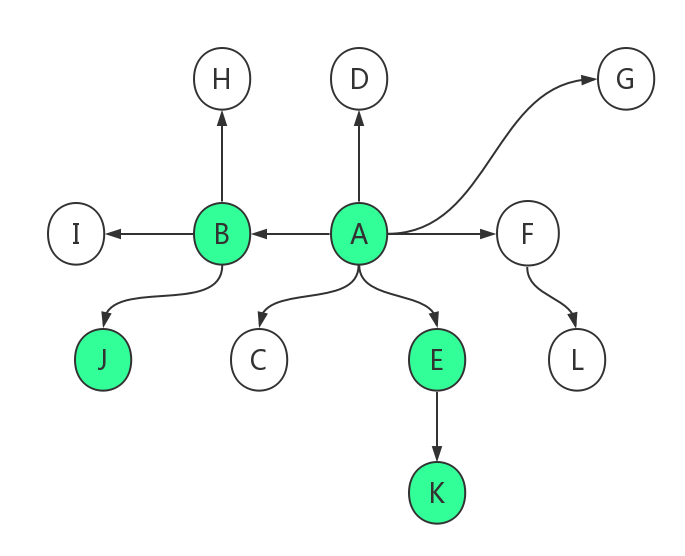
\includegraphics[width=0.5\textwidth]{USER}
    \bicaption{消息在用户网络上的传播过程}{The spread of news on the user's network}
    \label{fig:user}
\end{figure}

\item 地域特征反映了 Hashtag 存在明显的地理因素,不同地域的人关注的焦 点不同,因此具有明显的地域分布,结果展示如表\ref{tab:3_6_localtion}所示,某些主题标签带有明显的地域色彩,因此利用地域特征进行分组,形成 Hashtag 的局部聚类,有效 地表达了不同聚类结果。通过加入地域特征,可以将数据有效分组, 当去掉地域 特征以后,模型的性能下降很多,MAE 提高了 15.8\%,MSLE 提高了 16\%。
\begin{table}[H]
\newcommand{\tabincell}[2]{\begin{tabular}{@{}#1@{}}#2\end{tabular}}
    \centering
    \footnotesize% fontsize
    \bicaption{主题标签的地域特征}{Geographical characteristics of topic labels}
      \label{tab:3_6_localtion}
    \setlength{\tabcolsep}{8pt}% column separation
    \renewcommand{\arraystretch}{1.2}%row space 
    \begin{tabular}{c|c|c}
        \hline
       \textbf{ 地区} & \textbf{具体地区}& \textbf{Hashtag } \\
        %\cline{2-9}% partial hline from column i to column j
        \hline
		\textbf{海外} &中国以外的其他国家& \tabincell{c}{韩国水晶防晒喷雾,\\龟岛,龟梨和也} \\ \hline
		\textbf{东三省}&黑龙江, 吉林, 辽宁 & \tabincell{c}{二人转, 雾凇岛,\\冰雪大世界} \\ \hline
		\textbf{西北}& 青海, 新疆, 宁夏, 甘肃, 陕西& \tabincell{c}{羊肉泡馍, 青海湖旅游攻略\\西北贫困地区的孩子们一起成长} \\
        	\hline
    \end{tabular}
     
\end{table}


\item 主题特征对于 Hashtag 的预测十分重要, 当去掉主题特征时,模型的性能 下降很多,MAE 提高了 20\%,MSLE 提高了 18\%,反映出主题特征对于流行度 预测的重要性。不同 Hashtag 的主题特征如表3.11所示,从表中可知虽然是同一 个 Hashtag,但是随着时间的变化,其主题特征也会发生相应的变化,抽取不同 时刻的主题词来表示不同时刻的用户关注的焦点,对于主题标签的流行度预测 是具有重要参考价值的,因此刻画其主题特征是十分有必要的。

\begin{table}[H]
\newcommand{\tabincell}[2]{\begin{tabular}{@{}#1@{}}#2\end{tabular}}
    \centering
    \footnotesize% fontsize
    \bicaption{主题特征随着时间的变化
}{Topic features change over time}
      \label{tab:3_6_topic}
    \setlength{\tabcolsep}{6pt}% column separation
    \renewcommand{\arraystretch}{1.2}%row space 
    \begin{tabular}{c|c|c|c}
        \hline
       \textbf{ Hashtag} & \textbf{day-1 }& \textbf{day-2 }& \textbf{day-3}  \\
        %\cline{2-9}% partial hline from column i to column j
        \hline
		\textbf{文化新闻脱又秀} & \tabincell{c}{优酷, 分享, 新闻,
		\\故事, 沙和, 文化,
		\\微笑, 老师, 客户,
		\\一起, 看看} &  \tabincell{c}{今波, 贞观, 李世民,
		\\孟姜女哭, 土豆, 文化,
		\\天子, 新闻, 故事,
		\\什么, 中国, 下载} & \tabincell{c}{今波, 季-, 朱由校,
		\\秘招, 文化, 新闻,
		\\故事, 花絮, 独家,
		\\明朝, 皇帝, 救国,
		\\个人, 前世, 八仙,
		\\ 今生, 录制, 爱好, 中国}\\ \hline
		
		\textbf{周杰伦中国好声音} & \tabincell{c}{冯小刚, 声音, 大赞,
		\\领悟力, 宣传片, 给力,
		\\奥特曼, 才情, 满分,
		\\电影, 幽默, 合作} & \tabincell{c}{声音, 杰伦, 我的,
		\\偶像, 中国, 一直,
		\\我家, 歌词, 只有,
		\\随便, 超级, 长大,
		\\ 忘记, 出来, 好听} & \tabincell{c}{叶湘伦, 忽高,
		\\颜值, 只服, 周杰伦歌迷,
		\\后援会, 声音, 音乐,
		\\杰伦, 拜拜, 窒息,
		\\ 崩溃, 中国, 现场,
		\\赶往, 录制} \\ \hline
		
		\textbf{家族世代} & \tabincell{c}{信托, 视野, 观点,
		\\商界, 全球, 中外,
		\\大佬, 产品, 18 年,
		\\人物, 所有, 结果,
		\\默默无闻, 帝国} & \tabincell{c}{行善, 莫忘, 订阅,
		\\ 微信, 简史, 任正非,
		\\信托, 工具, 观点,
		\\斗争, 对方, 制度,
		\\迷茫, 政经, 技术} & \tabincell{c}{美国通用, 海尔, 惊天,
		\\马云, 王健林, 订阅,
		\\ 微信, 5 年, 56 亿美金,
		\\ 沉寂, 筹谋, 背后,
		\\故事, 年前, 人物} \\ 
        	\hline
    \end{tabular}
     
\end{table}

\end{enumerate}

在全部的特征集合上,本文衡量了全部特征重要性的集合,选取前 30 维最 重要的特征,如表\ref{tab:3_9}所示。通过对特征重要性的排序,本文发现时间序列是最 重要的,并且在整个时间序列特征中,开始时刻的时间序列特征是最重要的,反 映了开始时刻的长期影响,这个是本文的一个发现,并且通过选取前 30 维特征, 在可以牺牲一些精度的前提下,可以大幅度提高运算速度,对于后续优化提供了 思路。同时时间序列特征的效果最好,对整个预测任务最有用,这个是最重要的 特征,充分说明 Hashtag 存在明显的时间序列分布,对于后续 Hashtag 流行度的 预测提供了参考。另一方面,通过特征重要性的分析,可以看出本文针对主题标 签流行度预测提出的用户粉丝网络结构特征,主题特征,以及地域特征具有较高 的重要性,充分说明了该特征的有效性。



\begin{table}[H]
    \centering
    \footnotesize% fontsize
         \bicaption{ xgboost 特征重要性排序前三十维}{Xgboost feature importance prioritization of thirty dimensions}
      \label{tab:3_9}
    \setlength{\tabcolsep}{15pt}% column separation
    \renewcommand{\arraystretch}{1.2}%row space 
    \begin{tabular}{cccc}
        \hline
        \textbf{Rank} &  \textbf{Feature} &\textbf{ Rank} & \textbf{Feature}  \\
        %\cline{2-9}% partial hline from column i to column j
        \hline

       1 & 时间序列特征 & 16 & 主题向量-第十二维 \\
       2 &省地域特征-第十维& 17& 主题向量-第十五维 \\
       3 &地区地域特征-第一维 & 18 &地区地域特征-第七维\\
      4 & 微博长度 &19 &  用户向量-第十维\\
       5 & 主题向量-第一维 &20 &    地区地域特征-第二维\\
       6 & 消息类型 &21 & 朋友数   \\
       7 & 主题向量-第五维 &22& 微博情感性\\
        8&      是否包含 URL &23 &   省地域特征-第三维 \\
             9&评论数 &24 & 地区地域特征-第六维  \\
       10 &       转发数 & 25 & 用户向量-第三十四维  \\
             11 &省地域特征-第二十维 &26 & 主题向量-第十九维 \\
       12 &       主题向量-第十维 &27 & 省地域特征-第九维 \\
       13&地区地域特征-第五维 &28 & 是否包含数字    \\
          14 &用户向量-第四维 &29 & 用户向量-第五十二维  \\
            15 & 粉丝数 &30 & 用户向量-第六十四维    \\



      
      
        	\hline
    \end{tabular}

\end{table}


\section{本章总结}
传统的主题标签流行度预测方法主要是基于时间序列特征,内容特征,很少 考虑主题标签的自身特性以及考虑消息在用户粉丝网络结构上的传播机制,因 此提出了一种基于多维度特征的主题标签流行度预测算法,基于用户粉丝网络 结构特征,刻画消息在用户之间的传播特性,时间序列特征,主题特征,地域特 征,Hashtag 自身特性以及用户特征等多系列不同维度的特征,结合 xgboost 机器 学习模型,得到了较好的流行度预测效果。同时本文对于提出的 Hashtag 自身特 性,地域信息以及用户粉丝网络结构特征的重要性进行了分析,实验结果表明添 加这几类新的特征以后,模型效果有了较大的提升,验证了这几类特征在主题标 签流行度预测上的重要性,对于后续主题标签流行度预测提供了新的研究方向。

